\PassOptionsToPackage{unicode, colorlinks=true, linkcolor=black, urlcolor=black}{hyperref}
\documentclass[t, table]{beamer}

%% load the theme with the correct option for your institute
%% currently supported are tudo and ethz
\usetheme{fact}

\usepackage[
  orientation=portrait,
  size=a0,
  scale=1.0,  % scale fonts with this factor
]{beamerposter}

\usepackage{fontspec}
\usepackage{polyglossia}
\setmainlanguage[variant=american]{english}

% microtypographic adjusments (protrusion, kerning etc.)
\usepackage{microtype}

% automatic enquoting depending on the language with \enquote{Bla}
\usepackage{csquotes}

% for the qrcode
\usepackage{qrcode}

% math setup
\usepackage{mathtools}
\usepackage{unicode-math}
\setmathfont[Scale=MatchLowercase]{TeX Gyre Pagella Math}

\usepackage{xfrac}
\usepackage[
  detect-weight=true,
  binary-units=true,
  per-mode=fraction,
  fraction-function=\sfrac
 ]
 {siunitx}
% some stupid sample text to fill the boxes
\usepackage{blindtext}

% offers the \begin{multicols}{NCOLS} environment
\usepackage{multicol}

% for including all types of graphics
\usepackage{graphicx}

\usepackage{tabularx}

% bibliography settings
\usepackage[
  backend=biber,
  style=numeric,
  url=false,
  sorting=none,
  firstinits=true,
]{biblatex}
\DeclareFieldFormat*{title}{\textit{#1}}


\newcommand{\stf}{\texttt{streams-framework} }
% a little complicated, but this creates an inline list.
\renewcommand*{\bibfont}{\footnotesize}
\addbibresource{references.bib}
\defbibenvironment{bibliography}
  {\noindent}
  {\unspace}
  {}
\renewbibmacro*{begentry}{%
  \usebeamercolor{bibliography item}%
  \color{bibliography item.fg}%
  \printtext[labelnumberwidth]{%
    \printfield{prefixnumber}%
    \printfield{labelnumber}%
  }%
  \setunit{\addnbspace}%
}
\renewcommand*{\finentrypunct}{\addperiod\space}

% just a helpful definition to get columns with a third of the textwidth
\newlength{\thirdtextwidth}
\setlength\thirdtextwidth{0.333333\textwidth}


\title{Distributed real-time data stream analysis for CTA}
\author{Kai Brügge and Alexey Egorov}
\newfontfamily{\firathin}{fira sans thin}
\usetikzlibrary{calc}
\usetikzlibrary{shadows.blur}

\begin{document}%

\begin{multicols}{2}
    \begin{block}[equal height group=B]{CTA - The Cherenkov Telescope Array}%
      \begin{multicols}{2}
        \begin{figure}
          \includegraphics[width=\linewidth]{images/cta.png}\\
          % \caption{The FACT Telescope during a calibration procedure \cite{fact-performance}}
        \end{figure}
        \columnbreak
        Once completed, the  Cherenkov Telescope Array (CTA)  will be able to map the gamma-ray sky
        in a wide energy range from several tens of GeV to some hundreds of TeV and will be more sensitive
        than previous experiments by an order of magnitude.

        CTA will consist of approximately 100 telescopes of different sizes and designs.
        Telescope data will be streamed via network from the telescopes to a central computing facility
        on-site.
      \end{multicols}
    \end{block}%

    \begin{block}[equal height group=A]{Monitoring the Gamma-Ray SKY}%
      \begin{multicols}{2}
        \begin{figure}
          \includegraphics[width=\linewidth]{figures/fermi.pdf}\\
          % \caption{Toller Plot.\cite{fact-performance}}
        \end{figure}
        \columnbreak
        One of CTA's main goals is monitoring the sky for transient events. These include Gamma-Ray Burst (GRBs) events and
        Active Galactic Nuclei (AGNs).
        GRBs are believed to occur on massive merge events or star collapses.
        These events can show variable behavior in terms of both total brightness and spectral properties.
        To gain more understanding about the physics behind GRBs and AGN it is vital to perform multi-wavelengths observations.
        In case a sudden increase in  flux is detected CTA can alert other experiments to trigger observations in other wavelengths bands.
        The figure to the left shows all localized GRB events as triggered by the FERMI satellite.
      \end{multicols}
    \end{block}%
    %
    % \begin{block}[equal height group=B]{\stf}%
    %   \begin{multicols}{2}
    %     \begin{figure}
    %       \includegraphics[width=\linewidth]{images/cta.png}\\
    %       % \caption{The FACT Telescope during a calibration procedure \cite{fact-performance}}
    %     \end{figure}
    %     \columnbreak
    %       The \stf is a data streaming environment written in Java.
    %       The purpose of the streams-framework is to provide an abstract way to model the data flow of an application.
    %       It comes with a number of fundamental building blocks to define a data flow graph using an Extensible Markup Language (XML) based description.
    %       Programms written within the \stf can be executed on distributed computing engines such as Apache Storm, Flink and Spark.
    %   \end{multicols}
    % \end{block}%


    \begin{block}[equal height group=A]{Classification and Regression}%
      \begin{multicols}{2}
        \begin{figure}
          \includegraphics[width=\linewidth]{figures/ml_performance_multi_telescope_auc.pdf}\\
          % \caption{Toller Plot.\cite{fact-performance}}
        \end{figure}
        \columnbreak

        Supervised machine learning is used to separate signal from background and to estimate
        the energy of a recorded event. Features for classification/regression are calculated from raw input
        images.
        Simulated, labeled, data is used to train the models using the Python machine learning library scikit-learn\cite{sklearn}.
        The trained scikit-learn models are converted into the PMML\cite{pmml} format using the sklearn2pmml\cite{sklearn2pmml} library.
        This way the stored model can be shared
        between programming languages and applied to the data stream from the telescopes.
      \end{multicols}
    \end{block}%

    \begin{block}[equal height group=A]{Framework Comparisons}%
      \begin{multicols}{2}
        \begin{figure}
          \includegraphics[width=\linewidth]{figures/runtime.png}\\
          % \caption{Toller Plot.\cite{fact-performance}}
        \end{figure}
        \columnbreak
        At the time of writing we that the streaming capabilities of the Apache Spark framework lack proper support and documentation
        which is why we concentrated on Storm and Flink. We compare the runtime of Storm, Flink and the streams-framework in a local setup on a single
        core to measure the impact of the overhead these frameworks produce. The results can be seen on the image on the left.
        There is no clear preference between Storm and Flink when it comes to runtime overhead. We chose to continue our experiments on
        Apache Flink due to easier setup, better visualization tools and a more comfortable abstraction compared to the rather low-level
        API of Apache Storm.
      \end{multicols}
    \end{block}%


% ------------------Next columns -----------------
% ------------------------------------------------
    \columnbreak

        \begin{center}

        \begin{streamblock}[equal height group=C, width=0.8\linewidth]{0mm}{-5mm}{}%
          \begin{multicols}{2}
            \begin{figure}
              \includegraphics[width=\linewidth]{figures/image.pdf}
            \end{figure}
            \columnbreak
            Images from all telescopes in the array get collected into a central trigger where images belonging together are merged into so called events.
            This way each image gets a unique event id.
            CTA emits up to \num{15 000} events per second\cite{trigger}.
          \end{multicols}
        \end{streamblock}%

        \begin{streamblock}[height=2cm, width=0.8\linewidth]{-5mm}{-5mm}{}%
          \begin{center}
            Distribute images Images throughout cluster
          \end{center}
        \end{streamblock}%

        \begin{streamblock}[equal height group=C, width=0.8\linewidth]{-5mm}{-5mm}{}%
          \begin{multicols}{2}
            \rowcolors{2}{gray!25}{white}
            {\color{maincolor}
            \begin{tabularx}{\linewidth}{cccc}
              \rowcolor{gray!50}
                \textbf{Length} \textbf{Width} & \textbf{Size} & \textbf{EventID} \\
                30 & 15   & 100   & 1\\
                40 & 10  & 200  & 1\\
                29 & 25  & 75  & 1\\
                40 & 30  & 500 & 3\\
                5 & 2  & 12 & 5\\
                20 & 13  & 84 & 3
            \end{tabularx}
            }

            \columnbreak
            Each image in the event has to be converted into feature representation before classification and regression.
            Due to the parallel nature of the processing, the processed images do not necessarily retain their order.
            At this stage per-telescope operations can be applied.

          \end{multicols}
        \end{streamblock}%

        \begin{streamblock}[equal height group=C, width=0.8\linewidth]{-5mm}{-5mm}{}%
          \begin{multicols}{2}
            \begin{figure}
              \includegraphics[width=\linewidth]{figures/ml_performance_auc_per_telescope.pdf}
            \end{figure}
            \columnbreak

            At this stage the pre-trained machine learning models can be applied since they
            have been trained on single telescpe data. The plot on th eleft shows the performance
            of background suppression for the single telescopes

          \end{multicols}
        \end{streamblock}%


        \begin{streamblock}[height=2cm, width=0.8\linewidth]{-5mm}{-5mm}{}%
          \begin{center}
            Collect results belonging to the same event using a fixed time window.
          \end{center}
        \end{streamblock}%

        \begin{streamblock}[equal height group=C, width=0.8\linewidth]{-5mm}{-5mm}{}%
          \begin{multicols}{2}
            \begin{figure}
              \includegraphics[width=\linewidth]{figures/angular_resolution_vs_energy.pdf}
            \end{figure}
            \columnbreak
            The direction of the air shower is reconstructed from the features calculated in the previous step.
            The plot on the left shows the angular resolution of the reconstruction for different energy bands.
          \end{multicols}
        \end{streamblock}%

        \begin{streamblock}[equal height group=C, width=0.8\linewidth]{-5mm}{-5mm}{}%
          \begin{multicols}{2}
            \begin{figure}
              \includegraphics[width=\linewidth]{figures/ml_performance_multi_telescope_auc.pdf}
            \end{figure}
            \columnbreak
            Predictions for the single telescopes are averaged to get a better predictor.
            The plot on the left shows the area under the reciever operating characteristic.
          \end{multicols}
        \end{streamblock}%

      \end{center}

\end{multicols}


\vfill
\begin{columns}[t, onlytextwidth]%
  \begin{column}{0.42\textwidth}%
    \begin{block}[equal height group=bottom]{\normalsize References}
      \footnotesize%
      \printbibliography%
    \end{block}
  \end{column}%
  \begin{column}{0.42\textwidth}%
    \begin{block}[equal height group=bottom]{\normalsize Acknowledgment}
      \begin{multicols}{2}%
        \footnotesize
        Part of this work is supported by Deutsche Forschungsgemeinschaft (DFG) within the Collaborative Research Center SFB 876
"Providing Information by Resource-Constrained Analysis", project C3. 

      \end{multicols}%
    \end{block}
  \end{column}%
  \begin{column}{0.16\textwidth}%
    \begin{block}[equal height group=bottom]{\normalsize Contact}
      \begin{columns}%
        \begin{column}{0.33\textwidth}
          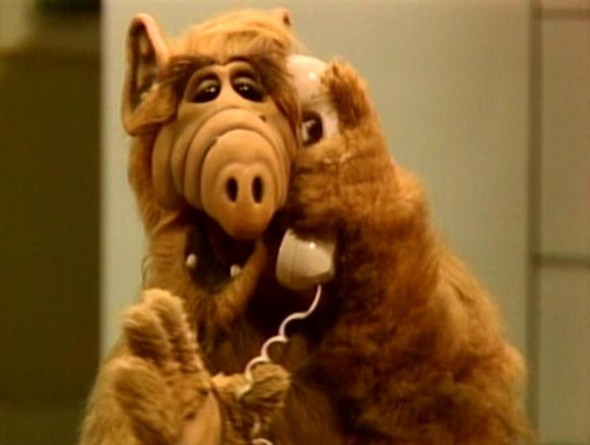
\includegraphics[width=\linewidth]{images/alf.jpg}
        \end{column}
        \begin{column}{0.65\textwidth}
          \footnotesize
              Kai Brügge, \\
              Astroparticle Physics, \\
              TU Dortmund \\
              \texttt{kai.bruegge@udo.edu}
        \end{column}

      \end{columns}
    \end{block}
  \end{column}%
\end{columns}%
\end{document}
